\begin{equation*}
% every colour follows the ink (white on the site's dark page, black in the PDF): the lanes mix green into the ink,
% the link boxes fill with green over the page, the ink's complement
\colorlet{lanecolor}{green!60!.}\colorlet{paper}{-.}%
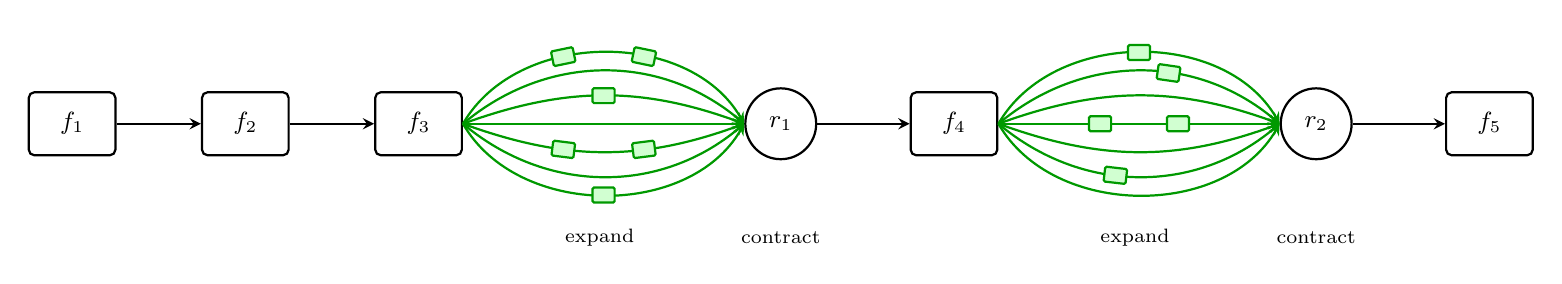
\begin{tikzpicture}[
  inst/.style={draw, rounded corners=2pt, thick, minimum width=11mm, minimum height=8mm, font=\small},
  fold/.style={draw, circle, thick, minimum size=9mm, font=\small},
  hop/.style={thick, ->, >=stealth},
  lane/.style={thick, ->, >=stealth, color=lanecolor},
  link/.style={draw=lanecolor, fill=green!18!paper, thick, rounded corners=0.5pt, minimum width=2.8mm,
               minimum height=1.9mm, inner sep=0pt},
  note/.style={font=\scriptsize}
]
\node[inst] (f1) at (0,0)   {$f_1$};
\node[inst] (f2) at (2.2,0) {$f_2$};
\node[inst] (f3) at (4.4,0) {$f_3$};
\draw[hop] (f1) -- (f2);
\draw[hop] (f2) -- (f3);
\node[fold] (r1) at (9.0,0) {$r_1$};
\foreach \ang in {-60,-40,-20,0,20,40,60}
  \draw[lane] (f3.east) to[bend left=\ang] (r1.west);
\path (f3.east) to[bend left=60] node[link, pos=0.38, sloped] {} node[link, pos=0.62, sloped] {} (r1.west);
\path (f3.east) to[bend left=20] node[link, pos=0.5, sloped] {} (r1.west);
\path (f3.east) to[bend left=-20] node[link, pos=0.35, sloped] {} node[link, pos=0.65, sloped] {} (r1.west);
\path (f3.east) to[bend left=-60] node[link, pos=0.5, sloped] {} (r1.west);
\node[inst] (f4) at (11.2,0) {$f_4$};
\draw[hop] (r1) -- (f4);
\node[fold] (r2) at (15.8,0) {$r_2$};
\foreach \ang in {-60,-40,-20,0,20,40,60}
  \draw[lane] (f4.east) to[bend left=\ang] (r2.west);
\path (f4.east) to[bend left=60] node[link, pos=0.5, sloped] {} (r2.west);
\path (f4.east) to[bend left=0] node[link, pos=0.35, sloped] {} node[link, pos=0.65, sloped] {} (r2.west);
\path (f4.east) to[bend left=-40] node[link, pos=0.42, sloped] {} (r2.west);
\path (f4.east) to[bend left=40] node[link, pos=0.6, sloped] {} (r2.west);
\node[inst] (f5) at (18.0,0) {$f_5$};
\draw[hop] (r2) -- (f5);
\node[note] at (6.7,-1.45)  {expand};
\node[note] at (9.0,-1.45)  {contract};
\node[note] at (13.5,-1.45) {expand};
\node[note] at (15.8,-1.45) {contract};
\end{tikzpicture}
\end{equation*}
